% !TeX spellcheck = en_US

\documentclass[document.tex]{subfiles}

\begin{document}
    \section{Regression Models}
    
    \subsection{Simple Linear Regression}

    \begin{frame}{Introductory Example}
        You recently inherited your grandfather's \textbf{10-year old 44 sqm apartment} but as you don't want to use it by your own, you decided to rent it. Unfortunately, you have \textbf{no experience in real estate} and therefore no clue what rental price would be appropriate for the apartment. For this reason, you \textbf{scraped the size and rental price of 40 surrounding apartments} from a web-based real state portal:
        
        \begin{table}
            \scalebox{0.8}{\begin{tabular}{crr}
\toprule
Apartment No. & Apartment Size & Rental Price \\
\midrule
            1 &          40.38 &       551.73 \\
            2 &          40.40 &       528.99 \\
            3 &          41.42 &       529.86 \\
          ... &            ... &          ... \\
           40 &          59.57 &       595.94 \\
\bottomrule
\end{tabular}
}
        \end{table}
        
        Unfortunately, none of the apartments in the dataset has a size of exactly 44 sqm. So, the central problem now is, \textbf{how can we learn a model to predict the rental price for the apartment as a function of its size}?

        \small{\href{https://nbviewer.jupyter.org/github/saschaschworm/big-data-and-data-science/blob/master/notebooks/demos/rental-prices-single-linear-regression.ipynb}{\textsc{\textbf{$\rightarrow$ open notebook in github}}}}
    \end{frame}

    \stepcounter{openexercise}
    \begin{frame}{Open Exercise \arabic{openexercise}}
        For our given problem here, what is the \textbf{learning task} and what is the \textbf{learning style}? Also state which variable is considered as the \textbf{feature} and which one as the \textbf{target}.
        
        \note{
            The learning style is \textbf{supervised} as we have target which is labeled and the learning task is \textbf{regression} as we want to predict a continuous outcome. The target here is the rental price and the feature is the apartment size.
            
        }
    \end{frame}

    \begin{frame}{Introductory Example Visualization}
        \begin{figure}
            \label{fig:rental-prices-slr-visualization}
            \includegraphics[width=\textwidth, keepaspectratio]{figures/rental-prices-slr-visualization.pdf}
        \end{figure}
    \end{frame}

    \begin{frame}{Training Set and Hypothesis}
        \begin{itemize}
            \item Let $x^{(i)}$ denote the \textbf{input variables (features)} and $y^{(i)}$ the \textbf{output variable (target)} where the superscript $(i)$ is an \textbf{index to the dataset} a machine learning algorithm is using, then a pair $(x^{(i)}, y^{(i)})$ is called a \textbf{training instance} and so a set of $m$ training instances is called \textbf{training set}.
            \item With a given training set we want to learn a function $h:x \mapsto y$ that is capable of \textbf{accurately predicting a specific outcome} for $y$. This function $h$ is called \textbf{hypothesis}.
            \item Different from a \textbf{statistical hypothesis} which is an explanation about the \textbf{relationship between data populations} that is interpreted probabilistically, a hypothesis in machine learning is a \textbf{model} that \textbf{approximates a target function} by \textbf{mapping inputs to outputs}. 
            \item The \textbf{space of possible hypothesis} that a model may represent is given by the choice as well as by the configuration of a machine learning algorithm.
            \item In order to actually perform supervised learning with a specific machine learning algorithm on the data, we must decide how to \textbf{represent a hypothesis mathematically}  so that a computer is able to work with.
        \end{itemize}
    \end{frame}

    \begin{frame}{Linear Regression Hypothesis}
        \begin{itemize}
            \item For our particular problem here, let's assume that there is a \textbf{linear relationship} between the apartment size and the rental price. Thus we can approximate $y$ as linear function of $x$ and so our hypothesis is as follows:
            
            $$\hat y = h(x) = \theta_0 + \theta_1x_1,$$
            
            with both $\theta_0$ and $\theta_1$ as its \textbf{parameters (or weight)} we want to learn (or estimate) with the aid of a machine learning algorithm and a given training set with features and a target variable.
            \item We can further simplify and generalize the above equation so it holds for linear regression models in general. Therefore, we can represent the \textbf{hypothesis for linear regression in general} by:
            
            $$\hat y = h(x) = \theta_0 + \theta_1x_1 + \dots + \theta_nx_n = \sum_{j=0}^n \theta_jx_j = \theta^Tx,$$
            
            where $n$ is the \textbf{number of features} (not counting for $x_0$) and where both $\theta$ and $x$ are viewed as \textbf{vectors}.
        \end{itemize}
    \end{frame}

    \begin{frame}{Loss Function}
        \begin{itemize}
            \item The \textbf{loss function} plays a \textbf{decisive role} in terms of learning the parameters of a hypothesis as it evaluates how well a learning algorithm models the given training set by continuously \textbf{measuring the inconsistency} between the predicted values for and the actual values of the target variable.
            \item This means that if for a given set of parameters the predictions deviate too much from the actual results, the loss function will output a higher number compared to predictions that are good.
            \item In \textbf{regression tasks}, one way to measure the inconsistency between the predicted and actual values is to calculate the \textbf{sum of squared errors} which is given by:
            
            $$SSE = \sum_{i=1}^m \epsilon^{(i)} = \sum_{i=1}^m (y^{(i)} - \hat y^{(i)})^2 = \sum_{i=1}^m (y^{(i)} - h(x^{(i)}))^2.$$
            
            \item To make the \textbf{math easier to handle} and the \textbf{derivative cleaner}, the $SSE$ is divided by 2 so that the 2 in the power gets canceled with the $\frac{1}{2}$ multiplier. Therefore, the final loss function is now given by:
            
            $$J(\theta) = \frac{1}{2} SSE = \frac{1}{2} \sum_{i=1}^m (y^{(i)} - h(x^{(i)}))^2.$$
        \end{itemize}
    \end{frame}

	\begin{frame}{Optimization}
		\begin{itemize}
			\item When we are speaking about supervised learning problems, we are basically just referring to \textbf{optimization problems} which seek to \textbf{minimize a corresponding loss function}.
			\item Minimizing the loss function basically means \textbf{finding feasible values} for all parameters of a hypothesis so that the \textbf{difference between the predicted and actual values is as small as possible} which in turn makes the output of the \textbf{loss function as small as possible} as well.
			\item To catch the idea behind it, imagine a \textbf{very simple yet inefficient method} for finding such a minimum: for every feasible set of parameters, calculate the corresponding output of the loss function and choose that combination which minimizes it. For only two sets of parameters we would obtain something as follows:
			\vspace{3mm}
			\begin{table}
				\scalebox{0.8}{\begin{tabular}{crrrrrr}
\toprule
 $i$ & $x^{(i)}$ & $y^{(i)}$ & $\hat y^{(i)}$ [I] & $\epsilon^{(i)}$ [I] & $\hat y^{(i)}$ [II] & $\epsilon^{(i)}$ [II] \\
\midrule
   1 &     40.38 &    551.73 &             203.90 &           120,985.71 &              285.66 &             70,793.24 \\
   2 &     40.40 &    528.99 &             204.00 &           105,618.50 &              285.80 &             59,141.38 \\
   3 &     41.42 &    529.86 &             209.10 &           102,886.98 &              292.94 &             56,131.09 \\
 ... &       ... &       ... &                ... &                  ... &                 ... &                   ... \\
  40 &     59.57 &    595.94 &             299.85 &            87,669.29 &              419.99 &             30,958.40 \\
\bottomrule
\end{tabular}
}
				\caption*{[I]: $\theta_0 = 2, \theta_1 = 5, J(\theta) = 1{,}905{,}671.3716$, [II]: $\theta_0 = 3, \theta_1 = 7, J(\theta) = 848{,}521.7830$}
			\end{table}
			\vspace{-5mm}
		\end{itemize}
	\end{frame}

    \begin{frame}{Loss Function Visualization}
        \begin{columns}
            \begin{column}{0.6\textwidth}
                \begin{itemize}
                    \item When doing those \textbf{calculations for many combinations}, we can get a glimpse on how the loss function for our particular rental price problem would look like in \textbf{3D space}.
                    \item Obviously, it is \textbf{not very efficient} (and actually not possible) to calculate the loss function output \textbf{for each and every parameter combination}.
                    \item Instead we want something that brings us from any given starting point on this \textbf{symbolical hill} right down to the \textbf{symbolical valley} as fast as possible.
                    \item As a computer cannot visually see the \textbf{path of steepest descent} down to the valley where our minimum is, we need something \textbf{mathematical} in combination with a specific \textbf{optimization algorithm} which gives us such a path.
                \end{itemize}
            \end{column}
            \begin{column}{0.4\textwidth}
                \begin{figure}
                    \label{fig:rental-prices-slr-loss-function-visualization}
                    \includegraphics[width=\textwidth, keepaspectratio]{figures/rental-prices-slr-loss-function-visualization.pdf}
                \end{figure}
            \end{column}
        \end{columns}
    \end{frame}

    \begin{frame}{Gradient Descent Intuition}
        \begin{columns}
            \begin{column}{0.6\textwidth}
                \begin{itemize}
                    \item Let's think of a a \textbf{hill climber} who wants to find a path which brings him from the \textbf{top of a mountain down to the valley} as fast as possible. As the \textbf{visibility is extremely low}, he only can use \textbf{local information} around him. 
                    \item Therefore, he repeatedly uses a \textbf{sophisticated instrument for measuring the steepness} of the hill at his current position and proceeds in the \textbf{direction with the steepest descent}.
                    \item As the \textbf{instrument is measuring quite slowly}, he wants to \textbf{minimize its usage} in order to arrive at the valley before sunset while keeping a \textbf{good frequency} that will not get him off the track.
                \end{itemize}
            \end{column}
            \begin{column}{0.4\textwidth}
                \begin{figure}
                    \label{fig:hill-climber-analogy}
                    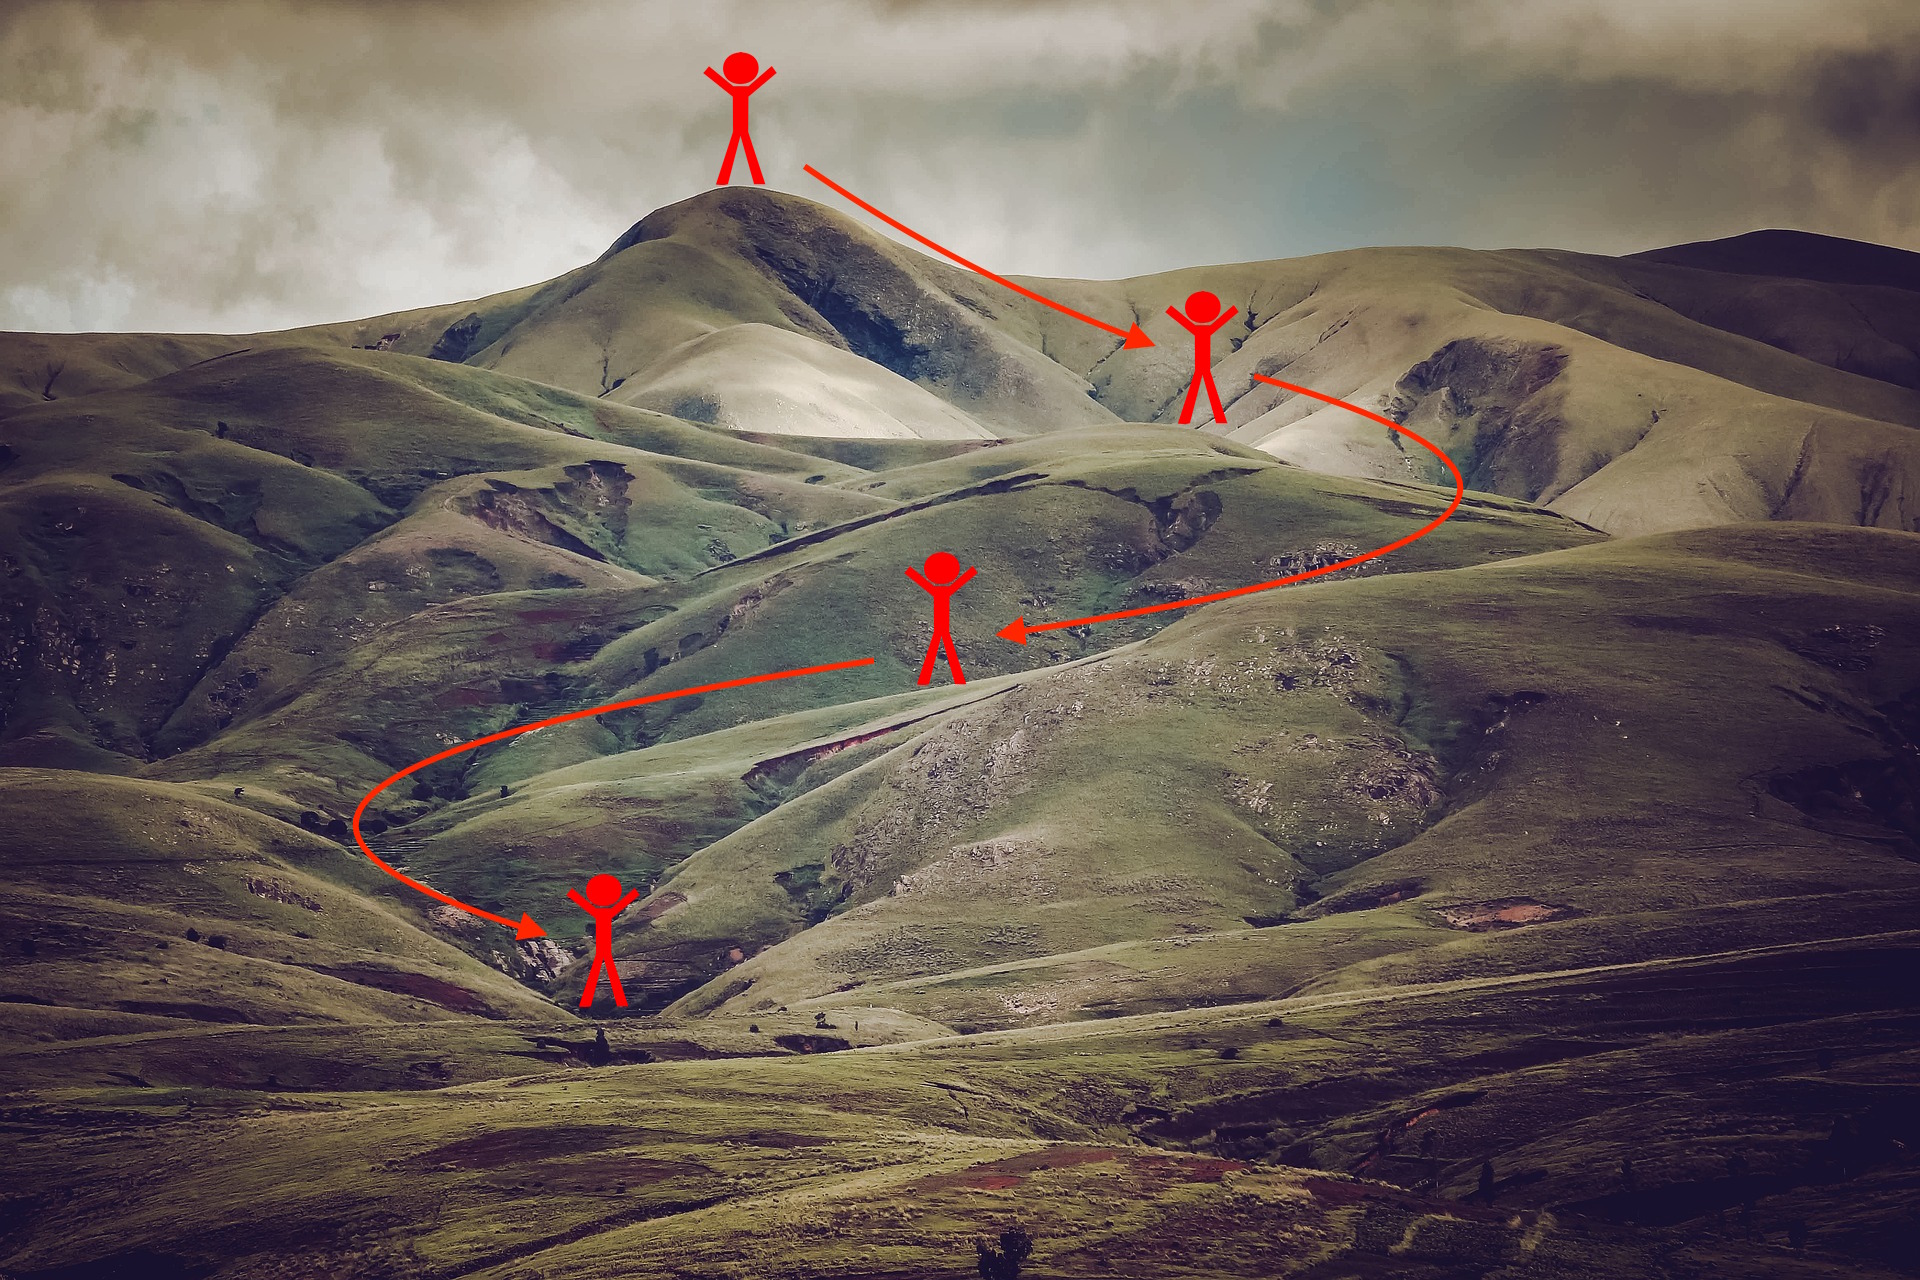
\includegraphics[width=0.9\textwidth, keepaspectratio]{figures/external/hill-climber-analogy.jpg}
                \end{figure}
            \end{column}
        \end{columns}
    \end{frame}

    \begin{frame}{Gradient}
        \begin{itemize}
            \item The \textbf{gradient} is a \textbf{differential operator} that assigns a multivariate function to its \textbf{first-order partial derivatives} and is therefore a \textbf{generalization of the derivative in multidimensional analysis}.
            \item With $\frac{\partial f}{\partial x_i}$ as the partial derivatives of $f$ and $\vec{e}_i$ as the \textbf{standard unit vectors} in the directions of the corresponding coordinate axes, the gradient is given by:
            
            $$\nabla f(x_1, \dots, x_n) = \frac{\partial f}{\partial x_1} \vec{e}_1 + \cdots + \frac{\partial f}{\partial x_n} \vec{e}_n = \begin{pmatrix}\frac{\partial f}{\partial x_{1}} \\ \vdots \\  \frac{\partial f}{\partial x_{n}} \end{pmatrix},$$
            
            \item The gradient of a \textbf{differentiable} multivariate function has the \textbf{direction of steepest increase} and thus the \textbf{negative gradient} has the \textbf{direction of the steepest decrease} of a function.
            \item The gradient just \textbf{points to the direction} and is \textbf{independent of the particular coordinate representation}. The same applies to the \textbf{magnitude} which is the \textbf{rate of increase/decrease} in that direction.
        \end{itemize}
    \end{frame}

    \begin{frame}{Exemplary Gradient Calculation}
        Given this simple function $f(x, y) = x^2 + y^2$, we want to find the \textbf{direction of steepest descent} for the randomly chosen point $P(-1|0)$. To do so, we initially must \textbf{calculate the partial derivatives} for $f$ which are given by $\frac{\partial f}{\partial x} = 2x$ and $\frac{\partial f}{\partial y} = 2y$ so that the gradient can be formulated as follows:
        
        $$\nabla f(x, y) = \frac{\partial f}{\partial x} \vec{e}_1 + \frac{\partial f}{\partial y} \vec{e}_2 =  2x \begin{pmatrix} 1 \\ 0\end{pmatrix} + 2y \begin{pmatrix} 0 \\ 1\end{pmatrix} = \begin{pmatrix} 2x \\ 0\end{pmatrix} + \begin{pmatrix} 0 \\ 2y \end{pmatrix} = \begin{pmatrix}2x \\ 2y \end{pmatrix}.$$
        
        With the gradient given, we can now \textbf{calculate the direction of the steepest descent} for our randomly chosen point $P$. As the \textbf{steepest decrease} is given by the \textbf{negative gradient}, we can calculate our final solution:
        
        $$-\nabla f(-1, 0) = -\begin{pmatrix}2 \cdot -1 \\ 2 \cdot 0 \end{pmatrix} = -\begin{pmatrix} -2 \\ 0 \end{pmatrix} = \begin{pmatrix} 2 \\ 0 \end{pmatrix}.$$
        
        \vspace*{-5mm}
    \end{frame}

    \begin{frame}{Gradient Field}
        What is displayed next is a \textbf{visualization of the previous example function} along with some \textbf{contour lines} as well as the corresponding \textbf{gradient field} with the gradients at various points:
        
        \begin{figure}
            \label{fig:gradient-field}
            \includegraphics[width=\textwidth, keepaspectratio]{figures/gradient-field.pdf}
        \end{figure}
        
        \vspace*{-3mm}
        We need now an \textbf{optimization algorithm} that actually follows those gradients and brings us all the way down to the valley where we will find the \textbf{optimal set of parameter} minimizing the loss function. 
    \end{frame}

    \begin{frame}{Gradient Descent}
        \begin{itemize}
            \item The \textbf{gradient descent} is an \textbf{iterative optimization algorithm} that uses the introduced concept of gradients in order to estimate the \textbf{optimal parameter values} for a hypothesis that minimize the loss function.
            \item The algorithm begins by \textbf{randomly choosing a vector of parameters} to start from. Those parameters are \textbf{unknown latent factors} so it is \textbf{useless to choose them in some predefined meaningful way}.
            \item Then the algorithm \textbf{repeatedly takes a step in the direction of steepest descent} and \textbf{updates the parameters} according to the \textbf{Widrow-Hoff learning rule} that for a single training instance is given by:
            
            $$\theta_j := \theta_j - \eta \frac{\partial J(\theta)}{\partial \theta_j} = \theta_j - \eta (y^{(i)} - h_\theta(x^{(i)}))x^{(i)}_j,$$
            
            with the \textbf{learning rate} $\pmb{\eta}$ as a special type of parameter called \textbf{hyperparameter}.
        \end{itemize}
    \end{frame}	

    \begin{frame}{Hyperparameters}
        \begin{itemize}
            \item Unlike the \textbf{standard model parameters} that get fit by training a model with a training set, \textbf{hyperparameters} cannot be learned from the regular training process and must be \textbf{fixed before} the actual process begins.
            \item Those hyperparameters express \textbf{higher-level properties of a model} such as its \textbf{complexity} or how many \textbf{iterations} a learning algorithm should run before stopping the training process. 
            \item The \textbf{actual number of hyperparameters} that can be adjusted beforehand \textbf{depend on the learning algorithm} that is used for training the model.
            \item The problem with hyperparameters is that there are \textbf{no magic numbers that work everywhere}. In fact, the best hyperparameter setting for a specific learning algorithm specifically depends on each textbf{learning task and on each dataset}.
            \item In one of the subsequent sections we will learn two approaches called \textbf{grid search} and \textbf{random search} that are part of a concept called \textbf{hyperparameter optimzation} that will helps us to solve the problem of choosing a set of optimal hyperparameters for a learning algorithm.
        \end{itemize}
    \end{frame}

    \begin{frame}{Learning Rate and Learning Rate Schedules}
        \begin{itemize}
            \item The \textbf{learning rate} $\pmb{\eta}$ is a hyperparameter that controls how much the algorithm adjusts the parameters on every step with respect to the gradient. In other words: it is \textbf{size of the steps} to take \textbf{in the direction of the steepest descent} of the loss function in any iteration.
            \item Setting the right learning rate introduces a \textbf{fundamental problem}: high values for the learning rate often lead to \textbf{overshooting or oscillation} around the minimum whereas very low values often \textbf{slowing down the process} of reaching the minimum and/or \textbf{trapping the algorithm} in an \textbf{undesirable local minimum}.
            \item So instead of using a \textbf{constant learning rate} for all iterations more often a \textbf{learning rate schedule} is used which changes the learning rate in each iteration with respect to a \textbf{adjustable decay or momentum factor} from a fixed initial value down to zero.
            \item One \textbf{major point of criticism with learning rate schedules} is that the factors like decay or momentum are \textbf{fixed beforehand} and so do \textbf{not adapt to the training set and to the learning process} in general which is a crucial point as especially the learning rate varies greatly depending on the problem and/or the model.
            \item As such, many \textbf{improvements on the basic gradient descent algorithm} have been proposed such as the \textbf{Adaptive Gradient Algorithm (AdaGrad)} or the \textbf{Adaptive Moment Estimation (Adam)} which implement an \textbf{adaptive learning rate} to combat the aforementioned problem.
        \end{itemize}
    \end{frame}

    \begin{frame}{Batches, Epochs and Iterations}
        \begin{itemize}
            \item As the gradient descent is an \textbf{iterative optimization algorithm} which means that in order to get the \textbf{best result} it is necessary to \textbf{pass over the training set for a multiple  of times} in a way that can also be controlled via a series of \textbf{additional hyperparameters}.
            \item A \textbf{batch} contains \textbf{one or more training instances} a learning algorithm has to work through before updating the parameters. The \textbf{actual number of instances in one batch} is set by a hyperparameter called \textbf{batch size}.
            \item One or more batches constitute one \textbf{epoch}, thus one epoch means that each batch and thus each training instance has had the \textbf{chance to update the model parameters}. The number of times a learning algorithm passes over the entire training set is also controlled by a specific hyperparameter - \textbf{the number of epochs}.
            \item \textbf{Iterations} refer to the \textbf{number of batches needed to complete one epoch}. For a training set with \textbf{1000 instances} and a \textbf{batch size to 250} it would take \textbf{4 iterations} to complete \textbf{1 epoch}.
        \end{itemize}
    \end{frame}

    \begin{frame}{Batch Gradient Descent}
        \begin{itemize}
            \item When generalizing the Widrow-Hoff learning rule for a \textbf{batch of $\pmb{m}$ training instances}, we finally obtain \textbf{one variant of the gradient descent algorithm} called the \textbf{batch gradient descent}:
            
            \begin{center}
                \begin{minipage}{.85\linewidth}
                    \begin{algorithm}[H]
                        \DontPrintSemicolon
                        \caption{Batch Gradient Descent}
                        Choose an initial vector of parameters and hyperparameters\;
                        \Repeat{an approximate minimum is obtained or a termination criterion is met}{
                            \lForEach{parameter $j$}{
                                $\theta_j := \theta_j - \eta \sum_{i=1}^m (y^{(i)} - h_\theta(x^{(i)}))x^{(i)}_j$
                            }
                        }
                    \end{algorithm}
                \end{minipage}
            \end{center}
            
            \vspace*{2mm}
            \item As the batch gradient decent passes over the entire training set before taking only a single small step in the direction of steepest descent, it is a very \textbf{costly operation} especially if the training set is large.
            \item Another \textbf{problem with gradient descent algorithms} in general and with the batch gradient descent in particular is that they are \textbf{susceptible to local minima}.
        \end{itemize}
    \end{frame}	

    \begin{frame}{Sample Optimization with Batch Gradient Descent}
        Exemplary Training Set: $S = ((2, 4), (4, 8))$ \\
        Underlying (but unknown) relation: $y = f(x) = 0 + 2x$ \\
        Initial (hyper)parameters: $\theta_0=1, \theta_1=3, \eta = 0.01$ \\
        Initial loss function value: $J(\theta) = \frac{1}{2} \sum_{i=1}^m (\theta_0 + \theta_1x_1^{(i)} - y^{(i)})^2 = 0.5 \cdot [(1 + 3 \cdot 2 - 4)^2 + (1 + 3 \cdot 4 - 8)^2] = 17$
        
        \begin{alertblock}{\textsc{Epoch 1}}
            Update rule: $0.01 \cdot [2 \cdot (4 - (1 + 3 \cdot 2)) + 4 \cdot (8 - (1 + 3 \cdot 4))] = -0.26$ \\
            Updated parameters: $\theta_0 := 1 + (-0.26) = 0.74, \theta_1 := 3 + (-0.26) = 2.74$ \\
            Updated loss function value: $J(\theta) = 0.5 \cdot [(0.74 + 2.74 \cdot 2 - 4)^2 + (0.74 + 2.74 \cdot 4 - 8)^2] = 9.3092$
        \end{alertblock}
        
        \begin{alertblock}{\textsc{Epoch 2}}
            Update rule: $0.01 \cdot [2 \cdot (4 - (0.74 + 2.74 \cdot 2)) + 4 \cdot (8 - (0.74 + 2.74 \cdot 4))] = -0.1924$ \\
            Updated parameters: $\theta_0 := 0.74 + (-0.1924) = 0.5476, \theta_1 := 2.74 + (-0.1924) = 2.5476$ \\
            Updated loss function value: $J(\theta) = 0.5 \cdot [(0.5476 + 2.5476 \cdot 2 - 4)^2 + (0.5476 + 2.5476 \cdot 4 - 8)^2] = 5.0977$
        \end{alertblock}
        
        \begin{alertblock}{\textsc{Result after Epoch 19}}
            $\theta_0 := 0.0024, \theta_1 := 2.0024, J(\theta) = 0.0001$ \\
        \end{alertblock}
    \end{frame}

    \begin{frame}{Convexity, Local and Global Optima}
        \begin{columns}
            \begin{column}{0.6\textwidth}
                \begin{itemize}
                    \item A function is said to be \textbf{strictly convex} if it is possible to \textbf{trace a line between any two of its points without crossing the function line}.
                    \item Strict convexity ensures that the only \textbf{local optimum of a function is global} at the same time. \item So if a loss function is convex (which is the case in linear regression), the gradient descent algorithm will \textbf{converge} but for \textbf{non-convex loss functions} the gradient descent algorithm might get \textbf{trapped into a local minimum}.
                    \item Adding some \textbf{stochastic randomness} to the batch gradient descent algorithm can help jumping out of a local into a global minimum.
                \end{itemize}
            \end{column}
            \begin{column}{0.4\textwidth}
                \begin{figure}
                    \label{fig:convexity}
                    \includegraphics[width=\textwidth, keepaspectratio]{figures/convexity.pdf}
                \end{figure}
            \end{column}
        \end{columns}	
    \end{frame}

    \begin{frame}{Stochastic Gradient Descent}
        \begin{itemize}
            \item The \textbf{stochastic gradient descent} passes multiple times over the training set which is \textbf{randomly shuffled in each epoch} and updates the parameters according to the gradient every time it encounters a \textbf{batch of one training instance} only. The complete algorithm is as follows:
            
            \begin{center}
                \begin{minipage}{.9\linewidth}
                    \begin{algorithm}[H]
                        \DontPrintSemicolon
                        \caption{Stochastic Gradient Descent}
                        Choose an initial vector of parameters and hyperparameters\;
                        \Repeat{an approximate minimum is obtained or a termination criterion is met}{
                            Randomly shuffle instances in the training set\;
                            \For{$i$ \KwTo $m$}{
                                \lForEach{parameter $j$}{
                                    $\theta_j := \theta_j - \eta (y^{(i)} - h_\theta(x^{(i)}))x^{(i)}_j$
                                }
                            }
                        }
                    \end{algorithm}
                \end{minipage}
            \end{center}
        
            \vspace*{2mm}
            \item This algorithm has not only \textbf{much lower computational costs compared to batch gradient descent} but also gives the path it wanders over more places and thus is \textbf{more likely to escape from a local minimum}.
        \end{itemize}
    \end{frame}	

    \begin{frame}{Termination Criteria}
        \begin{itemize}
            \item We already figured \textbf{two scenarios} in which a gradient descent algorithm might not converge to the global minimum. This can happen either if the \textbf{learning rate is too high} or if the \textbf{loss function is not convex}.
            \item Especially for those cases the gradient descent algorithm requires some \textbf{termination criteria} (which are basically further hyperparameters) in order to prevent an \textbf{endless looping}.
            \item The most obvious one here with regards to the stochastic gradient descent is to set a \textbf{maximum number of passes over the entire training set} which is a hyperparameter we already defined as the \textbf{number of epochs}.
            \item Another way to stop the gradient descent algorithm from endlessly looping is to define a \textbf{tolerance level)} which causes the algorithm to stop iterating whenever the loss function value of $\pmb{z}$ \textbf{consecutive epochs} is higher than the \textbf{best loss function value} minus the value set as tolerance level.
            \item Like with all hyperparameters, \textbf{setting the right termination criteria is more art than science} and nothing but the data only dictates what is wrong and what is right.
        \end{itemize}
    \end{frame}

    \begin{frame}{Python Implementation: Simple Linear Regression I/II}
        \lstinputlisting[language=Python, style=material]{snippets/rental-prices-slr-fitting-1.py}
    \end{frame}
    
    \begin{frame}{Python Implementation: Simple Linear Regression II/II}
        \lstinputlisting[language=Python, style=material]{snippets/rental-prices-slr-fitting-2.py}
    \end{frame}
    
    \begin{frame}{Rental Price Problem Solution (Single Linear Regression)}
        \begin{figure}
            \label{fig:rental-prices-slr-solution}
            \includegraphics[width=\textwidth, keepaspectratio]{figures/rental-prices-slr-solution.pdf}
        \end{figure}
    
        With the estimated parameters, we can now formulate the model as $\hat y = h(x) = 0.24 + 10.95 \cdot x$ and are able to determine the optimal rental price setting $x = 44$ so that $\hat y = h(44) = 0.25 + 10.9.5 \cdot 44 = 482.01$ EUR.
    \end{frame}
    
    \begin{frame}{Root Mean Squared Error (RMSE)}
        \begin{itemize}
            \item To be better interpret the resulting value of our loss function we can transform it into a more descriptive measure which is called the \textbf{Root Mean Squared Error (RMSE)} and given by:
            
            $$RMSE = \sqrt{\frac{1}{m} \sum_{i=1}^m (y^{(i)} - h(x^{(i)}))^2}.$$
            \item As the \textbf{sum of squared errors} we have been used as loss function previously already has been divided by 2 we can derive the $RMSE$ for a particular example so that 
            
            $$RMSE = \sqrt{\frac{2J(\theta)}{m}} = \frac{2 \cdot 44,950.53}{40} = 47.4081,$$
            
            which means that the \textbf{average difference between the observed and predicted} rental price on the training set is around 33.53 EUR. Whether this is a\textbf{ good or bad prediction error} heavily depends on the \textbf{training set} itself but also on the \textbf{domain knowledge} and \textbf{business expertise}. 
        \end{itemize}
    \end{frame}

    \begin{frame}{Python Implementation: Root Mean Squared Error}
        \lstinputlisting[language=Python, style=material]{snippets/rental-prices-slr-rmse.py}
    \end{frame}

    \begin{frame}{Generalization}
        \begin{itemize}
            \item So far we used the \textbf{features and the actual values of the target} in our \textbf{training set} for learning, let the resulting model making \textbf{predictions on the features of the training set} and then \textbf{compared the predicted values with the actual values} of the target in order to \textbf{evaluate the performance} of our model.
            \item If the model has had a set of \textbf{features and the actual values of the target when learning} and it gets the \textbf{same features afterwards for prediction} now without the target, then it might \textbf{remember from learning} what the actual values of the target had been for the respective features and outputs those which would \textbf{heavily bias the performance measures} we have calculated so far.
            \item As we care about \textbf{generalization} and the \textbf{performance on future unseen data} we must follow a different approach in order to get a more \textbf{robust performance measure} for evaluating models.
        \end{itemize}
    \end{frame}

    \begin{frame}{Holdout Method}
            So instead of using the complete data as the training set we split the data into a \textbf{training and test (or validation) set}, let the model \textbf{learn only with the training set} and then let it \textbf{predict with the unseen features of the test set}. This form of validation is called \textbf{holdout method}.

            \begin{figure}
                \label{fig:rental-prices-slr-holdout-method}
                \includegraphics[width=.8\textwidth, keepaspectratio]{figures/rental-prices-slr-holdout-method.pdf}
            \end{figure}
            
            This \textbf{prevents the model from remembering features} it has already seen and therefore gives us a much \textbf{better idea} how well a model generalizes to unseen data.
    \end{frame}

    \begin{frame}{Python Implementation: Holdout Method}
        \lstinputlisting[language=Python, style=material]{snippets/rental-prices-slr-holdout-method.py}
    \end{frame}
    
    \begin{frame}{k-Fold Cross-Validation}
        Due to the \textbf{random allocation of observations} into the training and test set, the way how the data is \textbf{partitioned} might be extremely \textbf{unlucky}. One possible solution to address this problem is to use a method called \textbf{k-Fold Cross-Validation} which \textbf{repeats the process} a several number of times and \textbf{averages the results} at the end.
        
        \begin{center}
            \begin{minipage}{.85\linewidth}
                \begin{algorithm}[H]
                    \DontPrintSemicolon
                    \caption{k-Fold Cross-Validation}
                    Divide data into $k$ folds with approximately equal distribution of cases\;
                    \ForEach{fold $k_i$ in the $k$ folds}{
                        Set fold $k_i$ as the test set\;
                        Train model on the remaining $k-1$ folds\;
                        Evaluate model performance on fold $k_i$
                    }
                    Calculate average performance over $k$ folds
                \end{algorithm}
            \end{minipage}
        \end{center}
    \end{frame}

    \begin{frame}{10-Fold Cross-Validation Visualization}
        \begin{figure}
            \label{fig:rental-prices-slr-kfold}
            \includegraphics[width=\textwidth, keepaspectratio]{figures/rental-prices-slr-kfold-method.pdf}
        \end{figure}
    \end{frame}

    \begin{frame}{Python Implementation: k-Fold Cross-Validation}
        \lstinputlisting[language=Python, style=material]{snippets/rental-prices-slr-kfold-method.py}
    \end{frame}

    \begin{frame}{Prediction Error}
        \begin{figure}
            \label{fig:rental-prices-slr-residuals}
            \includegraphics[width=\textwidth, keepaspectratio]{figures/rental-prices-slr-residuals.pdf}
        \end{figure}
    \end{frame}

    \begin{frame}{Underfitting}
		\begin{itemize}
            \item A \textbf{good model generalizes well} from the training data to any data from the problem domain which in turn allows to make \textbf{predictions on future data} the model has never seen.
            \item If a model has both a \textbf{high error in the training set and a high error in the test set} then the model is said to be \textbf{underfitting} and therefore not a suitable model for prediction.
            \item Underfitting simply means that a \textbf{model does not fit the data well enough}. This is because the model is \textbf{unable to capture the relationship} between the training instances and the target values causing a \textbf{high bias} due to \textbf{erroneous assumptions in the hypothesis}.
            \item Getting \textbf{more training data will not help} to overcome underfitting. Instead the model should be \textbf{sufficiently complex} which is accomplished by adding \textbf{new features} or create \textbf{features from existing ones}.
        \end{itemize}
    \end{frame}
    
    \subsection{Polynomial Regression}
    
    \begin{frame}{Polynomial Regression}
        \begin{columns}
            \begin{column}{0.6\textwidth}
                \begin{itemize}
                    \item In our previous example we have seen that our model is \textbf{underfitting} which means that the \textbf{assumption of a linear relationship} between the features and the target \textbf{might not hold true}. 
                    \item To overcome underfitting, we might need to \textbf{increase the complexity} and hence choose a model that is able to \textbf{better capture the underlying relationship in the data than the simple linear regression} did.
                    \item What we want to use now is an \textbf{extension to simple linear regression} in which the relationship between the feature and the target is modeled as an \textbf{higher-degree polynomial} in the feature which gives the \textbf{polynomial regression} its name.
                    \vspace{1mm}
                    
                    \small{\href{https://nbviewer.jupyter.org/github/saschaschworm/big-data-and-data-science/blob/master/notebooks/demos/rental-prices-polynomial-regression.ipynb}{\textsc{\textbf{$\rightarrow$ open notebook in github}}}}
                \end{itemize}
            \end{column}
            \begin{column}{0.4\textwidth}
                \begin{figure}
                    \label{fig:polynomials}
                    \includegraphics[width=\textwidth, keepaspectratio]{figures/polynomials.pdf}
                \end{figure}
            \end{column}
        \end{columns}
    \end{frame}

    \begin{frame}{Polynomial Regression Hypothesis}
        \begin{itemize}
            \item Like simple \textbf{linear regression}, which is basically a \textbf{1st degree polynomial regression}, assumes a \textbf{linear relationship} between the feature and the target, a \textbf{2nd degree polynomial regression} assumes a \textbf{quadratic relationship} and a \textbf{3rd degree polynomial regression} assumes a cubic relationship and so on. Overall, the generalized hypothesis for polynomial regression is given as follows:
            $$h(x) = \theta_0 + \theta_1x_1 + \theta_2x_1^2 + \dots + \theta_nx_1^n,$$
            where $n$ is the \textbf{degree of the polynomial} which we consider as an \textbf{optimizable hyperparameter} as we only care about \textbf{excellent out-of-sample predictions} and not about \textbf{economically justifyable assumptions} about the \textbf{real relationship} among feature and target.
            \item However, the \textbf{training error} tends to \textbf{decrease as we increase the degree of the polynomial} where at the same time the \textbf{test error} tends to \textbf{decrease} down to a certain point after it \textbf{starts increasing again}.
            \item We now want to learn a polynomial regression model where the \textbf{degree of the polynomial} is initially and randomly set to \textbf{3}. Therefore, we first need to \textbf{transform} our initial dataset.
        \end{itemize}
    \end{frame}

	\stepcounter{devexercise}
    \begin{frame}{Development Exercise \arabic{devexercise}}
        \begin{alertblock}{\textsc{Task}}
            Use the following code snippet to transform the apartment size feature into a 3rd degree polynomial as well as the previous code snippets for single linear regression in order to learn a polynomial regression model.
            \lstinputlisting[language=Python, style=material]{snippets/rental-prices-pr-transformation.py}
        \end{alertblock}
        \begin{alertblock}{\textsc{Question}}
            What is the average root mean squared error on both the training and test sets obtained from 10-fold cross validation and what is conspicuous about it?
        \end{alertblock}
        \note{
            The average root mean squared error on the training sets is \textbf{155,072,833,004,037,312.00 EUR} and on the test sets \textbf{157,317,771,079,220,768.00 EUR} which is even worse than our \textbf{baseline simple linear regression} where the results have been 47.28 EUR on the training sets and 45.58 EUR on the test sets.
            
            \small{\href{https://nbviewer.jupyter.org/github/saschaschworm/big-data-and-data-science/blob/master/notebooks/development-exercises/polynomial-transformation.ipynb}{\textsc{\textbf{$\rightarrow$ open notebook in github}}}}

        }
    \end{frame}

    \begin{frame}{Scale Invariance}
        \begin{columns}
            \begin{column}{0.6\textwidth}
                \begin{itemize}
                    \item Whenever \textbf{features are highly varying in magnitudes, units and range} (which is the case here due the to polynomial transformation) the loss function surface would be a very \textbf{high curvature ellipse}.
                    \item As gradient descent algorithms without adaptive learning rate do not possess the \textbf{property of scale invariance}, they ignore the curvature and taking many steps which are not necessarily in the optimal direction because the \textbf{step size can be different} for each feature.
                    \item This means that \textbf{no matter how the learning rate is set} it is \textbf{either too small} and it will take a \textbf{long time} for the algorithm to converge or it is \textbf{too big} and the algorithm \textbf{never converges}.
                \end{itemize}
            \end{column}
            \begin{column}{0.4\textwidth}
                \begin{figure}
                    \label{fig:scale-invariance-curvature}
                    \includegraphics[width=0.8\textwidth, keepaspectratio]{figures/scale-invariance-curvature.pdf}
                \end{figure}
            \end{column}
        \end{columns}
    \end{frame}
    
    \begin{frame}{Normalization and Standardization}
        \begin{columns}
            \begin{column}{0.6\textwidth}
                \begin{itemize}
                    \item By \textbf{normalizing/standardizing} we can \textbf{reduce the curvature} and thus making the \textbf{surface more spherical} so that the \textbf{gradient points right at the minimum} which improves the overall convergence.
                    \item \textbf{Normalization} is the process of \textbf{rescaling features into a similar smaller range} such as -1.0 to 1.0 or 0.0 to 1.0 and is accomplished with:
                    $$X' = \frac{X - X_{MIN}}{X_{MAX} - X_{MIN}} \cdot (\lambda_{MAX} - \lambda_{MIN}) + \lambda_{MIN}.$$
                    \item \textbf{Standardization} refers to rescaling features to have a \textbf{mean of 0 and standard deviation of 1} and is accomplished with:
                    $$X' = \frac{X - \mu}{\sigma}.$$
                \end{itemize}
            \end{column}
            \begin{column}{0.4\textwidth}
                \begin{figure}
                    \label{fig:scale-invariance-sphere}
                    \includegraphics[width=0.8\textwidth, keepaspectratio]{figures/scale-invariance-sphere.pdf}
                \end{figure}
            \end{column}
        \end{columns}
    \end{frame}

    \begin{frame}{Python Implementation: Polynomial Regression with Normalization I/II}
        \lstinputlisting[language=Python, style=material]{snippets/rental-prices-pr-fitting-1.py}
\end{frame}

    \begin{frame}{Python Implementation: Polynomial Regression with Normalization II/II}
        \lstinputlisting[language=Python, style=material]{snippets/rental-prices-pr-fitting-2.py}
        Average RMSE on training and test set from baseline model (simple linear regression): 47.28/45.58 EUR.
    \end{frame}

    \begin{frame}{Error Scores for Different Polynomial Degrees}
        \begin{figure}
            \label{fig:rental-prices-pr-overfitting}
            \includegraphics[width=\textwidth, keepaspectratio]{figures/rental-prices-pr-overfitting.pdf}
        \end{figure}
    \end{frame}

    \begin{frame}{Overcomplexity}
        \begin{figure}
            \label{fig:rental-prices-pr-tradeoff}
            \includegraphics[width=\textwidth, keepaspectratio]{figures/rental-prices-pr-tradeoff.pdf}
        \end{figure}
    \end{frame}

    \begin{frame}{Overfitting}
        \begin{itemize}
            \item When a model is too complex and gets trained with too much features, it starts \textbf{learning from the noise and inaccurate data entries} in the dataset. This means that the \textbf{noise or random fluctuations} in the training data is \textbf{picked up and learned as concepts} by the model making it unrealistic.
            \item Whenever this occurs a model is said to be \textbf{overfitting} causing a \textbf{high variance} which is expressed by both a \textbf{low error in the training set and a high error in the test set} making the model not generalizing well.
            \item As such, many machine learning algorithms also include further \textbf{hyperparameters or techniques to limit and constrain} how much detail the model learns.
        \end{itemize}
    \end{frame}

    \stepcounter{openexercise}
    \begin{frame}{Open Exercise \arabic{openexercise}}
        Why does adding more diverse data to a training set might help to prevent overfitting?
    \end{frame}
    
    \note{
        More data means more \textbf{variation} which makes it harder for a machine learning to capture all this variation. It is unable to overfit all samples and is forced to \textbf{generalize} to make progress.
                
    }


    \begin{frame}{Regularization}
        \begin{itemize}
            \item Regularization adds a \textbf{cost term} to the loss function and therefore \textbf{penalizes the increasing model complexity} when bringing in more features. 
            \item In terms of regression, the most common regularization techniques are \textbf{LASSO (Least Absolute Shrinkage and Selection Operator, L1) regression} and \textbf{ridge regression (L2)}. 
            \item L1 adds the \textbf{absolute value of magnitude of coefficient} expressed by $\alpha \sum_{n}^{j} |\theta_j|$ as regularization term to the loss function whereas L2 adds the \textbf{squared magnitude of coefficient} expressed by $\alpha \sum_{n}^{j} \theta_j^2$.
            \item The \textbf{regularization rate} $\pmb{\alpha}$ is another \textbf{hyperparameter} that controls the \textbf{impact of the regularization term} on the overall loss function and therefore must be chosen carefully.
            \item If $\alpha$ is too high, the \textbf{model gets more simple (higher bias, lower variance)} and the \textbf{risk of underfitting increases} as the model won't learn enough about the training data.  If $\alpha$ is too low, the \textbf{model will be more complex (lower bias, higher variance)} and the \textbf{risk of overfitting increases} as the model learns too much about details and noise in the training data.
        \end{itemize}
    \end{frame}

    \begin{frame}{Python Implementation: LASSO and Ridge Regression}
        \lstinputlisting[language=Python, style=material]{snippets/regression-regularization.py}
    \end{frame}

    \begin{frame}{Regularizer Effects}
        \begin{figure}
            \label{fig:rental-prices-pr-regularization-effect}
            \includegraphics[width=\textwidth, keepaspectratio]{figures/rental-prices-pr-regularization-effect.pdf}
        \end{figure}
    \end{frame}
    
    \begin{frame}{Bias-Variance-Tradeoff I/II}
        \begin{columns}
            \begin{column}{0.6\textwidth}
                \begin{itemize}	
                    \item Models with \textbf{high bias} pay \textbf{little attention to the training data} and thus are oversimplified, which in turn leads to a \textbf{high error on training and test data}.
                    \item Models with \textbf{high variance} pay a lot of attention to training data and thus \textbf{not generalizing well on unseen data}, which in turn leads to a \textbf{good performance on training data} but has a \textbf{high error on test data}.
                    \item Overfitting and underfitting are the two biggest causes for poor performance of machine learning algorithms. \textbf{Underfitting} models have a \textbf{low variance} but a \textbf{high bias}, whereas \textbf{overfitting} models have \textbf{high variance} but a \textbf{low bias}. 
                \end{itemize}
            \end{column}
            \begin{column}{0.4\textwidth}
                \begin{figure}
                    \label{fig:bias-variance-tradeoff-1}
                    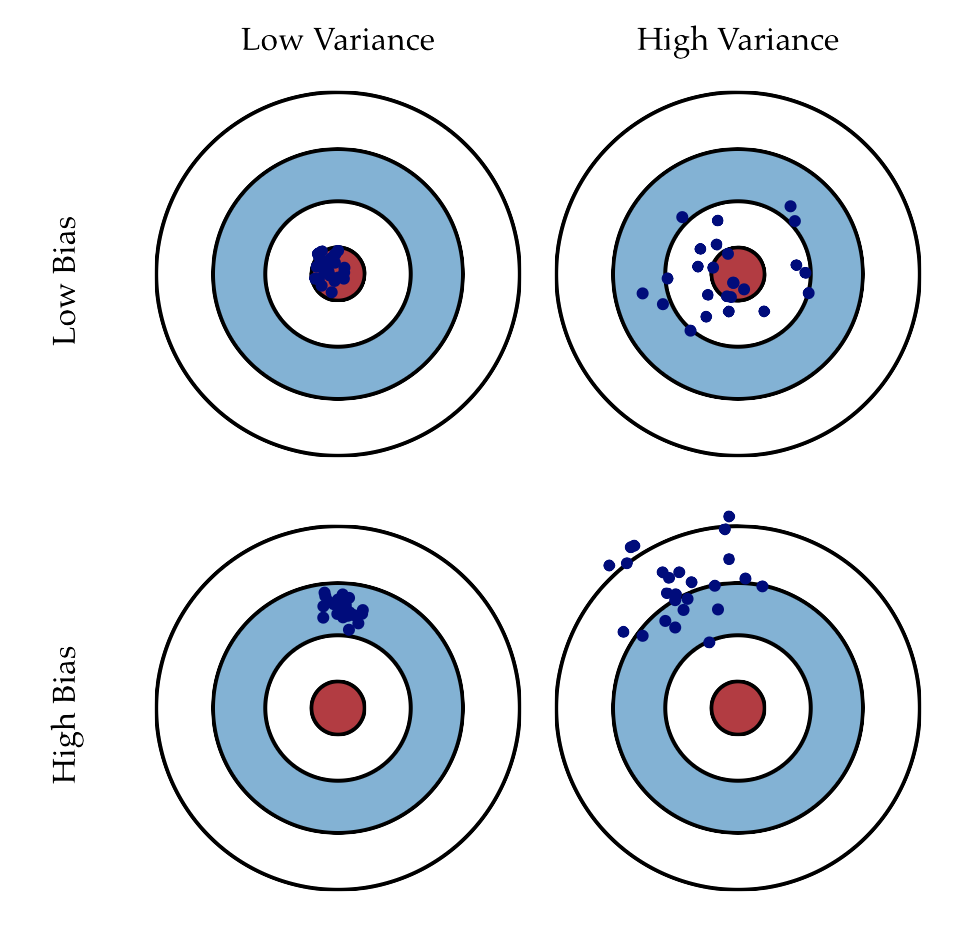
\includegraphics[width=\textwidth, keepaspectratio]{figures/external/bias-variance-tradeoff-1.png}
                \end{figure}
            \end{column}
        \end{columns}
    \end{frame}

    \begin{frame}{Bias-Variance-Tradeoff II/II}
        \begin{columns}
            \begin{column}{0.6\textwidth}
                \begin{itemize}	
                    \item To achieve \textbf{good prediction performance}, supervised machine learning models ideally should have a \textbf{low bias and a low variance}.
                    \item Unfortunately, there is no chance to escape the relationship between bias and variance as \textbf{increasing the bias} will \textbf{decrease the varianc}e and \textbf{increasing the variance} will \textbf{decrease the bias}. A model cannot simultaneously be \textbf{more complex and less complex}.
                    \item In reality, it is \textbf{not possible to calculate the real bias and variance error terms} because the \textbf{actual underlying target function is unknown}.
                \end{itemize}
            \end{column}
            \begin{column}{0.4\textwidth}
                \begin{figure}
                    \label{fig:bias-variance-tradeoff-2}
                    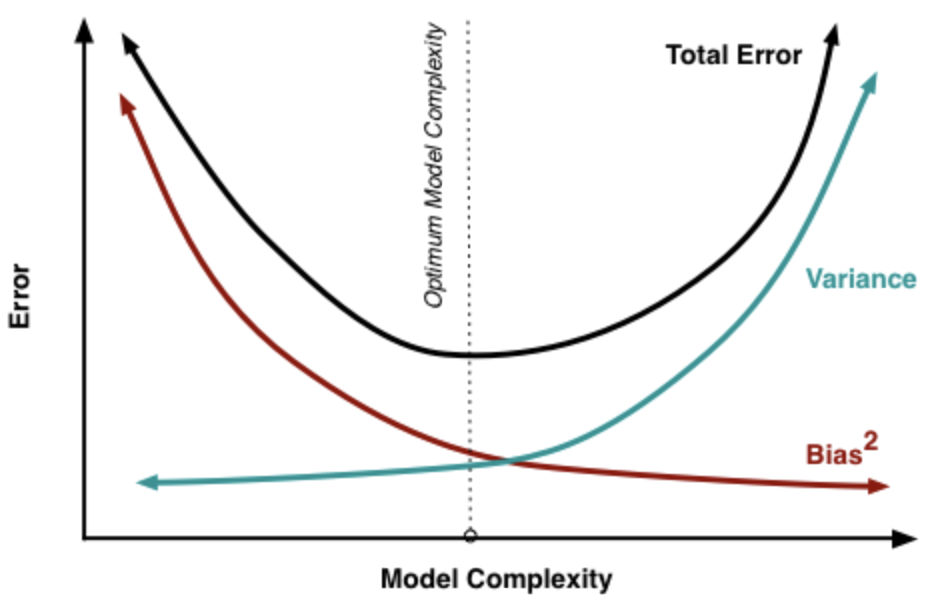
\includegraphics[width=\textwidth, keepaspectratio]{figures/external/bias-variance-tradeoff-2.png}
                \end{figure}
            \end{column}
        \end{columns}
    \end{frame}
        
    \subsection{Multiple Linear Regression}
    
    \begin{frame}{Introductory Example}
        Instead of using the same feature multiple times at different powers multiple regression explains the \textbf{relationship between the target variable and two or more different features}. Let's say we have not just collected the rental price and the apartment size but also the \textbf{number of years since construction} as well so that our dataset is like follows:

        \begin{table}
            \scalebox{0.8}{\begin{tabular}{crrr}
\toprule
Apartment No. & Apartment Size & Years since Construction & Rental Price \\
\midrule
            1 &          40.38 &                        5 &       551.73 \\
            2 &          40.40 &                        5 &       528.99 \\
            3 &          41.42 &                        8 &       529.86 \\
          ... &            ... &                      ... &          ... \\
           40 &          59.57 &                        5 &       595.94 \\
\bottomrule
\end{tabular}
}
        \end{table}

        How does this additional feature helps reducing the \textbf{unexplained variance} how does this affect the \textbf{prediction error} as well as the prediction itself?
        
        \small{\href{https://nbviewer.jupyter.org/github/saschaschworm/big-data-and-data-science/blob/master/notebooks/demos/rental-prices-multiple-linear-regression.ipynb}{\textsc{\textbf{$\rightarrow$ open notebook in github}}}}
    \end{frame}

     \begin{frame}{Multiple Linear Regression Hypothesis}
        \begin{itemize}        
            \item The \textbf{hypothesis for multiple linear regression} is the same as the \textbf{hypothesis for simple linear regression} we have already generalized in the previous subsections and therefore directly usable.
            \item For our particular problem now, the \textbf{hypothesis} would be now given by:
            $$y = h(x) = \theta_0 + \theta_1x_1 + \theta_2x_2,$$
            where $y$ is the apartment size, $x_1$ the rental price and $x_2$ the number of years since construction.
            \item The way how we can learn the parameters in multiple linear regression is also as same as for \textbf{simple linear regression} which means we can use the $SSE$ resp. the $MSE$ as loss function and the \textbf{stochastic gradient descent} for optimization.
        \end{itemize}
    \end{frame}

    \begin{frame}{Python Implementation: Multiple Linear Regression I/II}
        \lstinputlisting[language=Python, style=material]{snippets/rental-prices-mlr-fitting-1.py}
    \end{frame}

    \begin{frame}{Python Implementation: Multiple Linear Regression II/II}
        \lstinputlisting[language=Python, style=material]{snippets/rental-prices-mlr-fitting-2.py}
        Average RMSE on training and test set from baseline model (simple linear regression): 47.28/45.58 EUR.
    \end{frame}

    \stepcounter{devexercise}
    \begin{frame}{Development Exercise \arabic{devexercise}}
        \begin{alertblock}{\textsc{Task}}
            Use the age feature as well as the 21st degree polynomial of the apartment size feature to learn a multiple regression model with L1 regularization. Concerning the hyperparameters, set both regularization and learning rate to 0.0001 and the random state to 1909 to keep results comparable. All other should be set to default. Remember to normalize the numeric features!
        \end{alertblock}
        \begin{alertblock}{\textsc{Question}}
            What is the appropriate rental price for our 10-year old 44 sqm apartment with regards to the multiple linear regression model and what is the out-of-sample root mean squared error on both training and test sets using a 10-fold cross-validation?
        \end{alertblock}
        \note{
            The appropriate rental price for the 10-year old 44 sqm apartment is \textbf{515.35 EUR} and the average root mean squared error on the training sets is \textbf{22.32 EUR} and on the test sets \textbf{30.33 EUR} which is a great improvement compared to our \textbf{baseline simple linear regression} where the results have been 47.28 EUR on the training sets and 45.58 EUR on the test sets.
            
            \small{\href{https://nbviewer.jupyter.org/github/saschaschworm/big-data-and-data-science/blob/master/notebooks/development-exercises/rental-prices-multiple-linear-regression.ipynb}{\textsc{\textbf{$\rightarrow$ open notebook in github}}}}
            
        }
    \end{frame}

    \begin{frame}{Summary: Linear Regression}
        \begin{alertblock}{\textsc{Task and Type}}
            Supervised Machine Learning Model for Regression Tasks
        \end{alertblock}
        \begin{alertblock}{\textsc{Performance Measure}}
            Root Mean Squared Error (RMSE)
        \end{alertblock}
        \begin{alertblock}{\textsc{Strengths}}
            Straightforward to understand and explain; can be regularized to avoid overfitting; can be updated easily with new data using stochastic gradient descent; tends to have a low variance
        \end{alertblock}
        \begin{alertblock}{\textsc{Weaknesses}}
            Performs poorly on non-linear relationships; not flexible enough to capture complex patterns; choosing the right interaction terms and polynomials can be tricky and time-consuming; tends to have a high bias
        \end{alertblock}
    \end{frame}
    
    \subsection{Logistic Regression}
    
    \begin{frame}{Introductory Example}
        Let's suppose we have \textbf{historical data on this lectures exam results} and asked each student right after the exam has been written how many hours have been invested in learning and how many hours have been slept right before the exam:
           
        \begin{table}
            \scalebox{0.9}{\begin{tabular}{crrr}
\toprule
Student ID & Hours Studied & Hours Slept & Exam Passed \\
\midrule
         1 &        242.75 &        9.64 &           1 \\
         2 &        431.27 &        0.06 &           0 \\
         3 &        191.41 &        0.72 &           0 \\
       ... &           ... &         ... &         ... \\
       100 &        101.54 &        3.94 &           0 \\
\bottomrule
\end{tabular}
}
        \end{table}
    
        Based on the features given, we want to \textbf{predict for any future student} participating this course \textbf{whether or not he or she will pass the exam}. \textit{Remark: this data has been simulated and does not represent any real cases.}
        
        \small{\href{https://nbviewer.jupyter.org/github/saschaschworm/big-data-and-data-science/blob/master/notebooks/demos/exam-performance-logistic-regression.ipynb}{\textsc{\textbf{$\rightarrow$ open notebook in github}}}}
    \end{frame}

    \stepcounter{openexercise}
    \begin{frame}{Open Exercise \arabic{openexercise}}
        For our given problem now, what is the \textbf{learning task} and what is the \textbf{learning style}? Also state which variables are considered as the \textbf{features} and which one as the \textbf{target}.
        
        \note{
            The learning style is \textbf{supervised} as we have target which is labeled and the learning task is \textbf{classification} as we want to predict a discrete categorical outcome. The target here is the exam passed flag and the features are the hours studied and the hours slept.
            
        }
    \end{frame}

    \begin{frame}{Introductory Example Visualization}
        \begin{figure}
            \label{fig:exam-performance-visualization}
            \includegraphics[width=\textwidth, keepaspectratio]{figures/exam-performance-visualization.pdf}
        \end{figure}
    \end{frame}

	\begin{frame}{Logistic Function}
        \begin{itemize}
            \item In many classification problems, the target can take only two discrete values, 0 and 1. Those problems are called \textbf{binary classification problems} that cannot be addressed by linear regression models.
            \item Of course it is possible to ignore the fact, that the target is \textbf{discrete-valued} and thus use \textbf{linear regression models} but this method \textbf{performs very poorly} as several \textbf{assumptions are violated}.
            \item The idea therefore is to \textbf{squash the output of the linear regression hypothesis} into a \textbf{range between 0 and 1}. To do so, we make use of the \textbf{logistic (or sigmoid) function} which is given by:
            $$g(z) = \frac{1}{1 + e^{-z}}.$$
            \item A regression model that uses a logistic function to model a binary target is called \textbf{logistic regression model} which allows us to perform \textbf{classification tasks}.
        \end{itemize}
    \end{frame}

    \begin{frame}{Logistic Function Visualization}
        \begin{figure}
            \label{fig:sigmoid-function}
            \includegraphics[width=\textwidth, keepaspectratio]{figures/sigmoid-function.pdf}
        \end{figure}
    \end{frame}

    \begin{frame}{Logistic Regression Hypothesis}
        \begin{itemize}
            \item As the sigmoid function \textbf{maps any real value into another value between 0 and 1}, logistic regression \textbf{predicts the probability of occurrence of any binary event}, by using the following hypothesis:
            $$h(x) = g(\theta^Tx) = \frac{1}{1 + e^{-\theta^Tx}},$$
            where the output from the hypothesis is the \textbf{estimated probability}. For example, when the output is 0.75, we can say in terms of probability, that there is a 75\% chance that the student will pass the exam.
            \item As the hypothesis returns a probability score between 0 an 1, the \textbf{probability prediction must be transformed into a binary value} (0 or 1) in order to actually make a class predictions.
            \item Therefore we must set a \textbf{decision boundary} by selecting a \textbf{threshold value} (or tipping point) above which we classify probabilities into class 1 (exam failed) and below we classify values into class 2 (exam passed).
        \end{itemize}
    \end{frame}

    \begin{frame}{Cross-Entropy}
        \begin{itemize}
            \item In logistic regression, it is \textbf{not possible to use the mean squared error as loss function} as we did in linear regression because due to the sigmoid transformation, the \textbf{loss function is non-convex}.
            \item Therefore, \textbf{squaring the error results in a non-convex loss function} with \textbf{many local minimums}, which makes it more \textbf{difficult finding the optimal global minimum} during gradient descent.
            \item Instead of using the \textbf{MSE}, logistic regression uses the \textbf{Cross-Entropy}, also known as \textbf{Log Loss}, as the loss function which consists of two seperate loss functions, one for $y=1$ and one for $y=0$: 
            $$J(\theta)= \frac{1}{m} \sum_{i}^{m} C(h(x^{(i)}), y^{(i)}),$$
            where
            \[ C(h(x^{(i)}), y^{(i)})  =
            \begin{cases}
            -log(h(x^{(i)}))        & \quad \text{if } y^{(i)} = 1 \\
            -log(1 - h(x^{(i)}))    & \quad \text{if } y^{(i)} = 0
            \end{cases}.
            \]
        \end{itemize}
    \end{frame}

	\begin{frame}{Loss Function}
        \begin{itemize}
            \item Because of taking the logarithm, both loss function graphs are \textbf{smooth monotonic functions} (always increasing or always decreasing) making it \textbf{easy to calculate the gradient and to minimize the costs}.
        \end{itemize}
        \begin{figure}
            \label{fig:lr-loss-function-visualization}
            \includegraphics[width=.8\textwidth, keepaspectratio]{figures/lr-loss-function-visualization.pdf}
        \end{figure}
        \begin{itemize}
            \item Nevertheless, it is necessary to obtain one equation in order to solve for both $y=1$ and $y=0$ when using the gradient descent algorithm. By using the \textbf{Maximum Likelihood Estimation}, we obtain the final loss function:
            $$J(\theta)= -\frac{1}{m} \sum_{i}^{m} [y^{(i)}log(h(x^{(i)})) + 
            (1+^{(i)})log(1 - h(x^{(i)}))].$$
        \end{itemize}
    \end{frame}

    \begin{frame}{Python Implementation: Logistic Regression}
        \lstinputlisting[language=Python, style=material]{snippets/exam-performance-lr-fitting-1.py}
    \end{frame}

    \begin{frame}{Exam Performance Problem Solution I/II}
        \begin{figure}
            \label{fig:exam-performance-lr-solution-1}
            \includegraphics[width=\textwidth, keepaspectratio]{figures/exam-performance-lr-solution-1.pdf}
        \end{figure}
    \end{frame}

    \stepcounter{openexercise}
        \begin{frame}{Open Exercise \arabic{openexercise}}
        \begin{alertblock}{\textsc{Question}}
            What are the potential reasons our logistic regression classifier here behaves so bad in modeling the relationship between the features and the target and thus making so many misclassifications?
        \end{alertblock}
        \note{
            As the \textbf{logistic regression model} as we use it is a result of an \textbf{optimization with the gradient descent algorithm}, the \textbf{hyperparameters} might be not set correctly for this specific kind of problem and dataset. But what is more obvious here is that the bad performance is a \textbf{result of not-normalizing the features} that are highly varying in magnitude. 
            
        }
    \end{frame}

    \begin{frame}{Exam Performance Problem Solution II/II}
        \begin{figure}
            \label{fig:exam-performance-lr-solution-2}
            \includegraphics[width=\textwidth, keepaspectratio]{figures/exam-performance-lr-solution-2.pdf}
        \end{figure}
    \end{frame}

    \begin{frame}{Classification Metrics I/II}
        \begin{columns}
            \begin{column}{0.6\textwidth}
                \begin{alertblock}{\textsc{True Positives (TP)}}
                    Amount of samples that are \textbf{positive} \textit{(condition positive (P))} and have been \textbf{classified as positive}.
                \end{alertblock}
                \begin{alertblock}{\textsc{False Negatives (FN)}}
                    Amount of samples that are \textbf{positive} but have been \textbf{classified as negative}. This type of error is also called \textbf{Type II error}.
                \end{alertblock}
                \begin{alertblock}{\textsc{True Negatives (TN)}}
                    Amount of samples that are \textbf{negative} \textit{(condition negative (N))} and have been \textbf{classified as negative}.
                \end{alertblock}
                \begin{alertblock}{\textsc{False Positives (FP)}}
                    Amount of samples that are \textbf{negative} but have been \textbf{classified as positive}. This type of error is also called \textbf{Type I error}.
                \end{alertblock}
            \end{column}
            \begin{column}{0.4\textwidth}
                \begin{figure}
                    \label{fig:confusion-matrix}
                    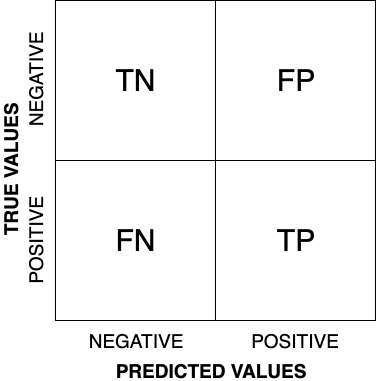
\includegraphics[height=0.8\textwidth, keepaspectratio]{figures/drawio/confusion-matrix.png}
                \end{figure}
            \end{column}
        \end{columns}
    \end{frame}

    \begin{frame}{Classification Metrics II/II}
        \begin{alertblock}{\textsc{Accuracy (ACC)}}
        The most common metric for classification is accuracy, which is the fraction of samples predicted correctly: $ACC = \frac{TP + TN}{P + N}$. Nevertheless, the accuracy is \textbf{not a reliable metric}, because it is heavily \textbf{biased if the dataset is imbalanced}.
        \end{alertblock}
        
        \begin{alertblock}{\textsc{Recall (True Positive Rate, TPR)}}
        The recall is the fraction of positives events that have been predicted correctly: $TPR = \frac{TP}{TP + FN}$. Recall shall be the model metric we use to select our best model when there is a \textbf{high cost associated with False Negative}.
        \end{alertblock}
        
        \begin{alertblock}{\textsc{Precision (Positive Predicitve Value, PPV)}}
        The precision is the fraction of predicted positives events that have been actually positive: $PPV = \frac{TP}{TP + FP}$. Precision is a good measure to determine, when the \textbf{costs of False Positive is high}.
        \end{alertblock}
        
        \begin{alertblock}{\textsc{F1 Score}}
        The F1 score is the harmonic mean of recall and precision: $F_1 = 2 \cdot \frac{PPV \cdot TPR}{PPV + TPR}$. F1 Score might be a better measure to use if we need to seek a \textbf{balance between Precision and Recall} and there is an \textbf{uneven class distribution}.
        \end{alertblock}
    \end{frame}

    \stepcounter{openexercise}
    \begin{frame}{Open Exercise \arabic{openexercise}}
        Think of real \textbf{business classification problems} and give one example each where \textbf{recall}, \textbf{precision} and \textbf{F1 score} would be an appropriate performance metric in order to evaluate a model.
    \end{frame}

    \note[itemize]{
        \item \textbf{Recall}: Fraud detection or sick-patient detection.
        \item \textbf{Precision}: Email spam detection.
        \item \textbf{F1 score}: Algorithmic trading.
        
    }

    \begin{frame}{Python Implementation: Classification Metrics I/II}
        \lstinputlisting[language=Python, style=material]{snippets/exam-performance-lr-classification-metrics-1.py}
    \end{frame}

    \begin{frame}{Python Implementation: Classification Metrics I/II}
        \lstinputlisting[language=Python, style=material]{snippets/exam-performance-lr-classification-metrics-2.py}
    \end{frame}

    \begin{frame}{Confusion Matrix}
        \begin{figure}
            \label{fig:exam-performance-lr-confusion-matrix}
            \includegraphics[height=.7\textheight, keepaspectratio]{figures/exam-performance-lr-confusion-matrix.pdf}
        \end{figure}        
    \end{frame}

    \begin{frame}{Multi-Class Logistic Regression}
        \begin{itemize}
            \item Logistic regression models are only binary classifiers which means that they \textbf{cannot handle target vectors with more than two classes}. One way to approach this is by using a \textbf{softmax function} instead of a \textbf{sigmoid function} for transformation. The resulting model is then called a \textbf{Multinomial Logistic Regression (or Softmax Regression)} model which we will not address here in this lecture.
            \item Another way to do multi-class logistic regression is to \textbf{re-run binary classification multiple times} once for each class. This approach is called \textbf{One-vs-Rest Logistic Regression (OVR)}, where a \textbf{seperate model is trained for each class} thus making it a binary classification problem again - one for each class.
            \item As each model in OVR predicts the probability whether an observation is in that class or not, the \textbf{class with the highest probability is selected} across among all model.
        \end{itemize}
    \end{frame}

    \stepcounter{devexercise}
    \begin{frame}{Development Exercise \arabic{devexercise}}
        \begin{alertblock}{\textsc{Task}}
            Lets suppose we have a student that has been learning for 4 hours and has been sleeping for 10 hours the night before the exam. Use the following code snippet to create a prediction dataset:
            \lstinputlisting[language=Python, style=material]{snippets/rental-prices-mlr-prediction-set.py}
            
            Use the following snippet to calculate a probability estimate:
            
            \lstinputlisting[language=Python, style=material]{snippets/rental-prices-mlr-prediction-probability.py}
        \end{alertblock}
        \begin{alertblock}{\textsc{Question}}
            Predict whether or not this student will pass the exam and give the corresponding probability estimate for it..
        \end{alertblock}
        \note{
            Prediction: 1, Probability Estimate: 90.10\%
            
            \small{\href{https://nbviewer.jupyter.org/github/saschaschworm/big-data-and-data-science/blob/master/notebooks/development-exercises/exam-performance-logistic-regression.ipynb}{\textsc{\textbf{$\rightarrow$ open notebook in github}}}}
            
        }
    \end{frame}

    \begin{frame}{Summary: Logistic Regression}
        \begin{alertblock}{\textsc{Task and Type}}
            Supervised Machine Learning Model for Classification Tasks
        \end{alertblock}
        \begin{alertblock}{\textsc{Performance Measure}}
            Accuracy, Logarithmic Loss, Area Under ROC Curve, Confusion Matrix
        \end{alertblock}
        \begin{alertblock}{\textsc{Strengths}}
            Easy robabilistic interpretation; can be regularized to avoid overfitting; can be updated easily with new data using stochastic gradient descent; tends to have a low variance
        \end{alertblock}
        \begin{alertblock}{\textsc{Weaknesses}}
            Tends to performs poorly when there are multiple or non-linear decision boundaries; not flexible enough to capture complex patterns; tends to have a high bias
        \end{alertblock}
    \end{frame}
\end{document}